\documentclass[12pt]{report}

%%%%%%%%%%%%%%%%%%%%%%%%%%
%%%%%% UNIT PREAMBLE %%%%% 
%%%%%%%%%%%%%%%%%%%%%%%%%%

% Basics 
\usepackage[utf8]{inputenc}
\usepackage[T1]{fontenc}
\usepackage{textcomp}
\usepackage[a4paper, left=1in, right=1in, top=1in, bottom=1in]{geometry}
\renewcommand\familydefault{\sfdefault}

\usepackage[Sonny]{fncychap}

\usepackage{amsmath,amsfonts,amsthm,amssymb,mathtools}
\usepackage[varbb]{newpxmath}
\usepackage{xfrac}
\usepackage[usenames,dvipsnames]{xcolor} % usenames, dvipsnames adds more colours
\usepackage{hhline}
\usepackage{comment}
\usepackage{tasks}
\usepackage{enumerate} 
\usepackage{enumitem} 
\usepackage{titlesec}
\usepackage[most]{tcolorbox}
\usepackage{lipsum}
\usepackage{tabularx}
\usepackage[labelfont=bf]{caption}
\usepackage{subfig}
\usepackage{pgfplots}
\usepackage{cancel} 
\usepackage{physics} 
\usepackage[bookmarks]{hyperref}
\usepackage{array}
\usepackage{float}
\usepackage{standalone}
\usepackage{graphicx}
\usepackage{forest}

% Tables 
\numberwithin{table}{section}

% Inkscape Figures
\usepackage{import}
\usepackage{xifthen}
\usepackage{pdfpages}
\usepackage{transparent}
\newcommand{\incfig}[2][1]{
    \def\svgwidth{#1\columnwidth}
    \import{../figures/}{#2.pdf_tex}
}

\pdfsuppresswarningpagegroup=1

% Chemistry
\usepackage{lewis} 
\usepackage{bohr}
\usepackage[version=4]{mhchem}

% Page setup
\hypersetup{hidelinks}
\pagenumbering{arabic}
\pagestyle{plain}
\setlength{\parindent}{0pt}

% Show subsubsections
\setcounter{tocdepth}{3}
\setcounter{secnumdepth}{3}

% Required for the Grid
\usetikzlibrary{calc}

% Section Font-Size
\titleformat{\subsubsection}
  {\normalfont\fontsize{12}{12}\bfseries}{\thesubsubsection}{1em}{}

\titleformat{\subsection}
  {\normalfont\fontsize{14}{14}\bfseries}{\thesubsection}{1em}{}

\titleformat{\section}
  {\normalfont\fontsize{16}{16}\bfseries}{\thesection}{1em}{}

% New page for each section 
\newcommand{\sectionbreak}{\clearpage}

% Section Spacing
\titlespacing{\section}{0em}{2.5em}{1em}
\titlespacing{\subsection}{0em}{2.5em}{1em}
\titlespacing{\subsubsection}{0em}{2.5em}{1em}

% TABLE COLUMN SEPARATION (USES ARRAY PACKAGE)
% \renewcommand{\arraystretch}{1.8} % changes vertical space for each cell 
% \setlength{\tabcolsep}{18pt} % changes horizontal space for each cell
% \setlength{\arrayrulewidth}{0.25mm}

% TCOLORBOX 
% \newtcolorbox[auto counter, number within=section]{definition}{colback=white,title=Example~\thetcbcounter,breakable,colframe=white,boxrule=0pt, enhanced, title style={left color=gray!60,right color=white,middle color=white},arc=0mm, titlerule=0pt, fonttitle=\bfseries\sffamily}

% Theorems 
\usepackage{thmtools}
\usepackage[framemethod=TikZ]{mdframed}

\declaretheoremstyle[
    headfont=\bfseries\sffamily\color{ProcessBlue!70!black}, bodyfont=\normalfont,
    headpunct= :,
    mdframed={
        linewidth=2pt,
        rightline=false, topline=false, bottomline=false,
        linecolor=ProcessBlue, backgroundcolor=ProcessBlue!5,
        innerbottommargin=10pt
    } ]{note}

\declaretheoremstyle[
    headfont=\bfseries\sffamily\color{NavyBlue!70!black}, 
    bodyfont=\normalfont,
    % headpunct=,
    mdframed={
        linewidth=2pt,
        rightline=false, topline=false, bottomline=false, linecolor=NavyBlue, innerbottommargin=10pt
    }
]{solution}

\declaretheoremstyle[
    headfont=\bfseries\sffamily\color{Gray!70!black}, bodyfont=\normalfont,
    % headpunct= ,
    postheadspace=\newline,
    mdframed={
        linewidth=2pt,
        rightline=false, topline=false, bottomline=false,
        linecolor=Gray, backgroundcolor=Gray!5,
        innerbottommargin=10pt
    } ]{remark}

\declaretheoremstyle[
    headfont=\bfseries\sffamily\color{Fuchsia!70!black}, bodyfont=\normalfont,
    % headpunct= ,
    mdframed={
        linewidth=2pt,
        rightline=false, topline=false, bottomline=false,
        linecolor=Fuchsia, backgroundcolor=Fuchsia!5,
        innerbottommargin=10pt
    }
]{example}

\declaretheoremstyle[
    headfont=\bfseries\sffamily\color{Fuchsia!70!black}, 
    bodyfont=\normalfont,
    % headpunct= ,
    mdframed={
        linewidth=2pt,
        rightline=false, topline=false, bottomline=false,
        linecolor=Fuchsia,
    }
]{examplesolution}

\declaretheoremstyle[
    headfont=\bfseries\sffamily\color{black!70!black}, 
    bodyfont=\normalfont,
    mdframed={
        linewidth=1pt,
        rightline=false, topline=false, bottomline=false,
        linecolor=black,
    }
]{definition}

\declaretheorem[style=solution, name=Solution, numbered=no]{solution}

\declaretheorem[style=solution, name=Derivation, numbered=no]{derivation}

\declaretheorem[style=definition, name=Definition, numberwithin=chapter]{definition}

\declaretheorem[style=note, name=Note, numbered=no]{noteswap}
\newenvironment{note}[1]{\vspace{0.5em}\begin{noteswap}[#1]}{\end{noteswap}\vspace{0.5em}}

\declaretheorem[style=remark, name=Remark, numbered=no]{remarkswap}
\newenvironment{remark}{\vspace{0.5em}\begin{remarkswap}}{\end{remarkswap}\vspace{0.5em}}

\declaretheorem[style=example, name=Example, numbered=no]{exampleswap}
% \newenvironment{example}{\vspace{0.5em}\begin{exampleswap}}{\end{exampleswap}}

\declaretheorem[style=examplesolution, name=Solution, numbered=no]{examplesolutionswap}
\newenvironment{examplesolution}{\vspace{-2em}\begin{examplesolutionswap}}{\end{examplesolutionswap}}

% Enumerate environments 
\newenvironment{2qu}
{
\begin{enumerate}[label=(\alph*)]
}
{\end{enumerate}}

\newenvironment{3qu}
{
\begin{enumerate}[label=(\roman*)]
}
{\end{enumerate}}

% Normal Environments 
\newenvironment{list0.5}
{
\begin{enumerate}
\setlength\itemsep{0.5em}
}
{\end{enumerate}}

% \titleformat{\section}{\vbox{\rule{\linewidth}{0.8pt}}\bigskip\LARGE\bfseries}{\thesection}{1em}{}

\titleformat{\section}
  {\normalfont\Large\bfseries}{\thesection}{1em}{}[{\titlerule[0.8pt]}] % horizontal line below

% thmtools Environments
\newenvironment{problems}
{
    \subsection{Problems}
    \begin{enumerate}
    \setlength\itemsep{1em}
}
{\end{enumerate}}

\newenvironment{+problems}
{
    \subsubsection{Problems}
    \begin{enumerate}
    \setlength\itemsep{1em}
}
{\end{enumerate}}

\newenvironment{example}[1]
{
    \begin{exampleswap}
        #1
    \end{exampleswap}
    \begin{examplesolution}
}
{
\end{examplesolution}}

\newenvironment{2example}[1]
{
    \begin{exampleswap}[#1]
}
{
\end{exampleswap}}

% Managing Figures
\captionsetup{width=0.8\textwidth}
\renewcommand{\thefigure}{\arabic{chapter}.\arabic{figure}}

% TABLE
% \begin{table}[h!] % delete [h!] if there are bugs

%     %%% TABLE CONFIG %%% 
%     \renewcommand{\arraystretch}{1.5} % changes vertical space for each cell 
%     \setlength{\tabcolsep}{10pt} % changes horizontal space for each cell
%     \setlength{\arrayrulewidth}{0.25mm}

%     \begin{center}
%          title of the table \
%         \vspace{0.5em}
%         \begin{tabular}{|c|c|} % use r, l, c for right, left, center. use m{3cm} for middle width of 3cm, use  b{3cm} for bottom width of 3cm, and use p{3cm} for a top width of 3cm.  
%         \hline
%          &  \ % two columns corresponding to two c's
%         \hline
%          &  \ % second row
%         \hline
%         \end{tabular}
%     \end{center}
%     \caption{}
% \end{table}

% Symbols 
\newcommand{\z}{\mathbb{Z}}

\renewcommand{\l}{\ell}

% Formatting 
\newcommand{\invis}{\vphantom{Invisible Text}}
\newcommand{\divider}{\par\noindent\rule{\textwidth}{0.5pt}\vspace{0.4em}}

% Chemistry
% \newcommand{\2ch}[2]{\ce{#1}_{(#2)}}
% \newcommand{\io}[2]{\text{#1}^{#2}} 
% \newcommand{\2io}[3]{\text{#1}^{#2}_{#3}}


\begin{document}

\subsection{Respiratory System}
\begin{definition}[Respiratory System]
    Responsible for providing oxygen to the body and removing carbon dioxide from the body. See Figure \ref{fig:respiratory-system} (a).
\end{definition}

\begin{figure}[!htb] 
    \centering
    \subfloat[\centering The lungs are protected by ribs.]{{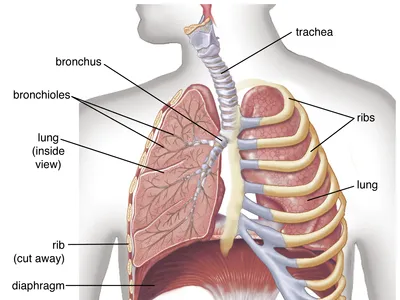
\includegraphics[width=0.45\textwidth]{../figures/respiratory system.png}}}  
    \qquad
    \subfloat[\centering The alveoli are in the lungs (search chatGPT for what this does).]{{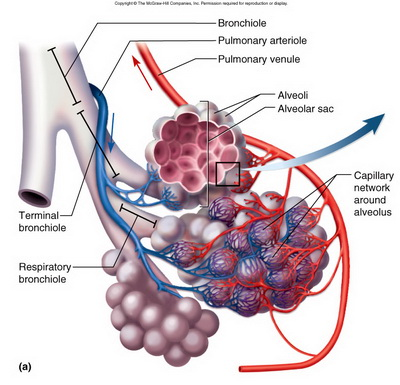
\includegraphics[width=0.45\textwidth]{../figures/alveoli.jpg}}}  
    % TODO
    \caption{The respiratory system.}
    \label{fig:respiratory-system}
\end{figure}

\subsection{Nose/Mouth}
\begin{definition}[Nose/Mouth]
    Where air enters and passes through the pharynx (throat). 
    \begin{itemize}
        \item{Mucous and hairs trap small particulates.}
        \item{Capillaries in the nose warm the air.}
    \end{itemize}
\end{definition}

\subsection{Larynx}
\begin{definition}[Larynx]
    For sound production and also functions to protect the lower airways by closing or coughing.
\end{definition}

\subsection{Trachea}
\begin{definition}[Trachea]
    The windpipe that is surrounded by cartilage rings to prevent collapse. The very top is the voice box, and it branches off into the bronchi, which eventually branches off into the lungs. See Figure \ref{fig:trachea}.
\end{definition}

\begin{figure}[H]
\centering
    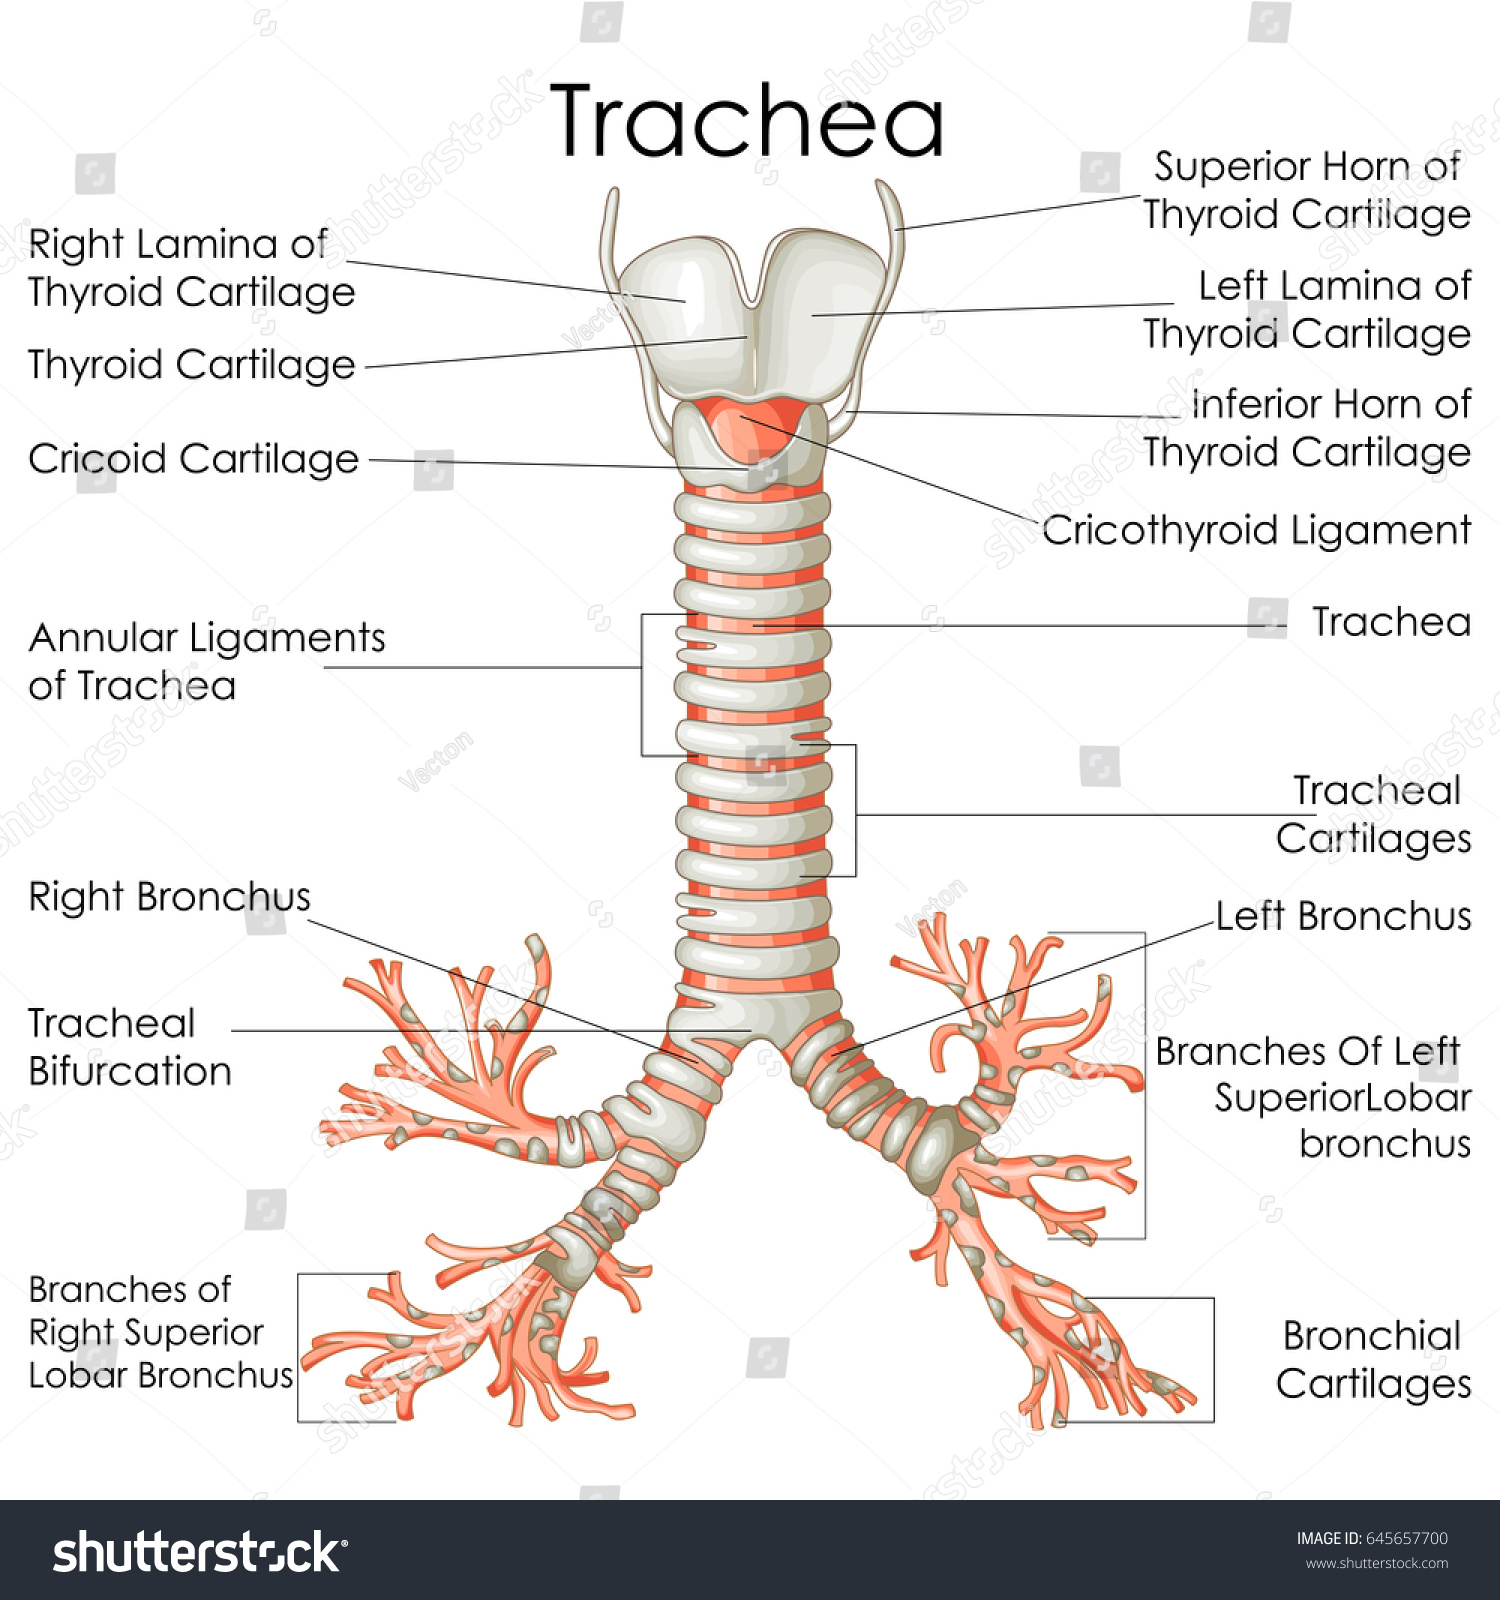
\includegraphics[width=0.5\textwidth]{../figures/trachea.jpg}
    \caption{The trachea branches off into the lungs.}
    \label{fig:trachea}
\end{figure}

\subsection{Bronchi}
\begin{definition}[Bronchi]
    Where the trachea splits into the left and right bronchus.
    \begin{itemize}
        \item{Contains goblet cells in the epithelial lining to produce mucus.}
        \item{Lined with cilia (hair-like projections) to sweep materials out of the lower airway.}
    \end{itemize}
\end{definition}

\subsection{Bronchioles}
\begin{definition}[Bronchioles]
    Where the bronhi splits into smaller tubes.
\end{definition}

\divider 

\subsection{In the Lungs: Alveoli}
\begin{definition}[In the Lungs: Alveoli]
    Tiny, capillary-bound sacs where gas exchange occurs between air and blood. See Figure \ref{fig:respiratory-system} (b) and Figure \ref{fig:alveoli}.
    \begin{itemize}
        \item{Membranes are thin to maximize diffusion.}
    \end{itemize}
    A better way to put it, from Figure \ref{fig:alveoli}, you can see that the alveoli and capillary are actually separated. How it works is that oxygen from the $ \text{bronchioles}\to \text{alveoli}$ gets diffused across and turns into carbon dioxide. Similarly, oxygen from the capillary itself gets diffused across and becomes deoxygenated as well.
\end{definition}

\begin{figure}[H]
\centering
    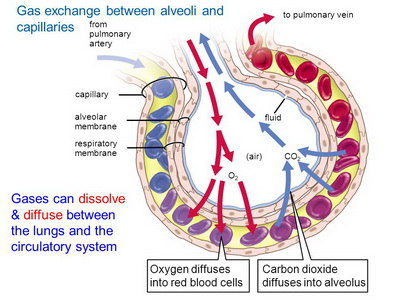
\includegraphics[width=0.7 \textwidth]{../figures/alveoli2.jpg}
    \caption{The oxygen diffuses (from blue to purple to red) and carbon dioxide is diffused out.}
    \label{fig:alveoli}
\end{figure}

\subsection{Pulmnary Arties and Capillaries}
\begin{definition}[Pulmnary Arties and Capillaries]
    Provides a large supply of deoxygenated blood to alveoli.
\end{definition}

\subsection{Pulmonary Veins}
\begin{definition}[Pulmonary Veins]
    Brings oxygenated blood back to the heart to be distributed to the rest of the blood.
\end{definition}

\subsection{Checkpoint: Pulmonary Fibrosis}
Pulmonary Fibrosis is when the tissue around the alveoli thickens and scars. How will this affet gas exchange?\\ 

\textbf{Solution:} The scar tissue will make gas exchange less efficient; this will result in a slowing down of the gas exchange, and will mean that the body's cells won't get rid of waste or get a delivery of oxygen as quickly as normal.

\subsection{Breathing}
\begin{definition}[Breathing]
    The process of breathing is caused by pressure differences between the atmosphere and the inside of the lungs.\\ 

    Air moves from an area of high pressure to low pressure.
    \begin{itemize}
        \item{Pressure can be changed by changing volume.}
            \begin{itemize}
                \item{Volume increases, pressure decreases. For example, imagine a balloon.}
                \item{Volume decreases, pressure increases.}
            \end{itemize}
    \end{itemize}
    The equation is $V\propto \frac{1}{p}.$
\end{definition}

\subsection{Lung Volume}
\begin{definition}[Lung Volume]
    Lung volume can be changed by: 
    \begin{itemize}
        \item{Contraction or relaxion of muscles in the rib cage.}
        \item{Contraction or relaxion of the \textbf{diaphragm,} which is a dome-shaped muscle underneath the lungs.}
    \end{itemize}
    In other words, when you inhale, the diaphragm compresses, and your lungs expand. When you exhale, this is when the diaphragm ``relaxes'', and is when it gets back into its normal shape, casugint he lungs to get smaller and greater air pressure within the lungs.
\end{definition}

\end{document}
